\section{One Class Reference}
\label{classOne}\index{One@{One}}
Inheritance diagram for One::\begin{figure}[H]
\begin{center}
\leavevmode
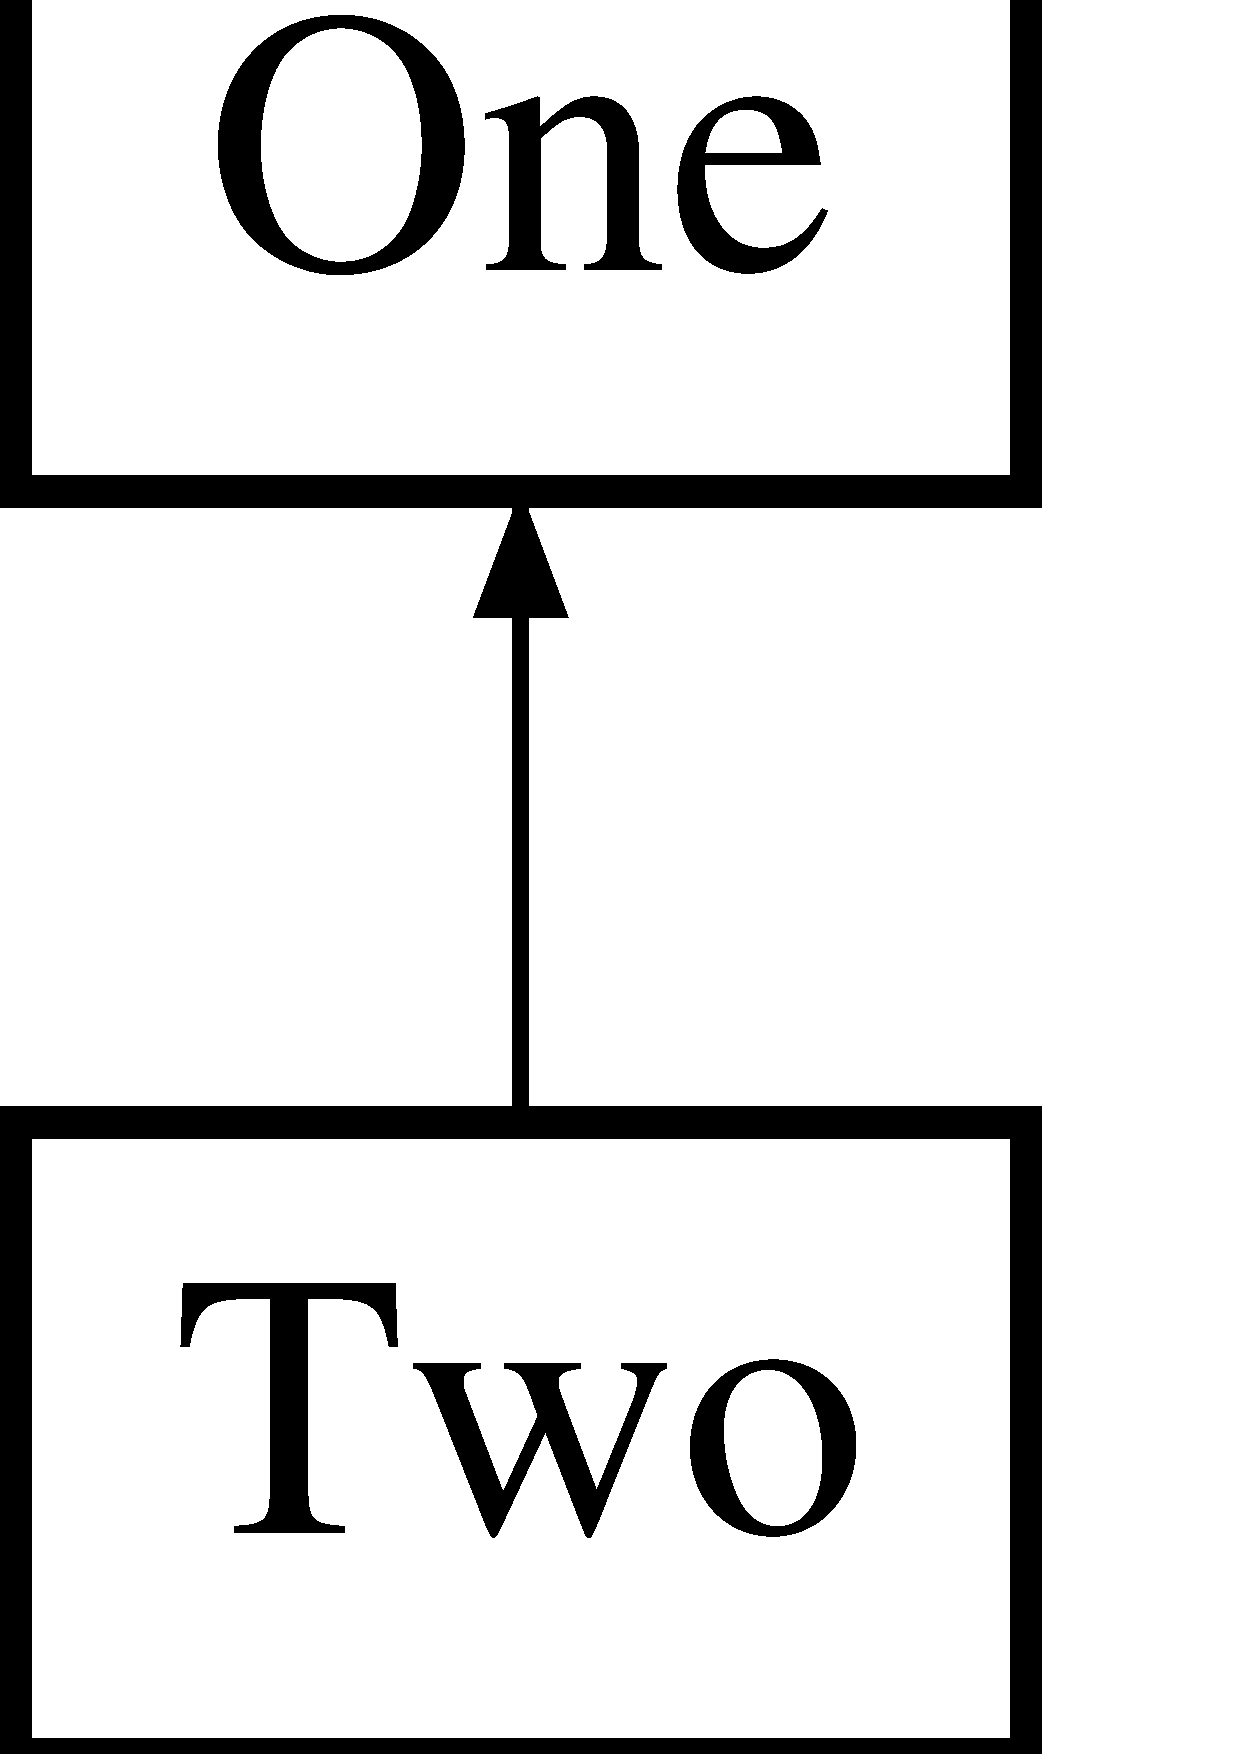
\includegraphics[height=2cm]{classOne}
\end{center}
\end{figure}
\subsection*{Static Public Member Functions}
\begin{CompactItemize}
\item 
static String {\bf get\-Text} ()\label{classOne_c400624dcb962b5eeb9f98630f48968e}

\item 
static int {\bf get\-Length} ()\label{classOne_e5dfb0ee9ca9b1b28c15d7bbf3fbea3f}

\end{CompactItemize}
\subsection*{Static Package Attributes}
\begin{CompactItemize}
\item 
static String {\bf text} = \char`\"{}Hey\char`\"{}\label{classOne_2443f2db7bdd17ccc5e650c3fd4e50ce}

\item 
static int {\bf length} = text.length()\label{classOne_a8e127d39c8e05f72c40f918c5290c2b}

\end{CompactItemize}


\subsection{Detailed Description}




Definition at line 13 of file Test\-Subclass\-Var\-Names.java.

The documentation for this class was generated from the following file:\begin{CompactItemize}
\item 
Test\-Subclass\-Var\-Names.java\end{CompactItemize}
